% !TeX encoding = UTF-8
% !TeX spellcheck = es_ES
% !TeX root = ../ComponentCatalog.tex
%!TEX root=../ComponentCatalog.tex

%Rocket KCD1-101
\begin{table}[H]
    \centering
    \renewcommand\theadfont{\bfseries}
    \setlength{\tabcolsep}{10pt}
    \renewcommand{\arraystretch}{1.6}

    \begin{tabular}{|c|c|c|c|c|}
        \beginConnectorTable{Interruptor Basculante}
        \multirow{4}{*}{\makecell{KCD1-101}}
        \connectordata{
            %\draw (0,0) rectangle  +(2.5,1.8);
            \begin{scope}
                \clip (0,0) rectangle  +(2.5,1.8);
                \node[inner sep=0pt] at (0.7,0.6)
                    {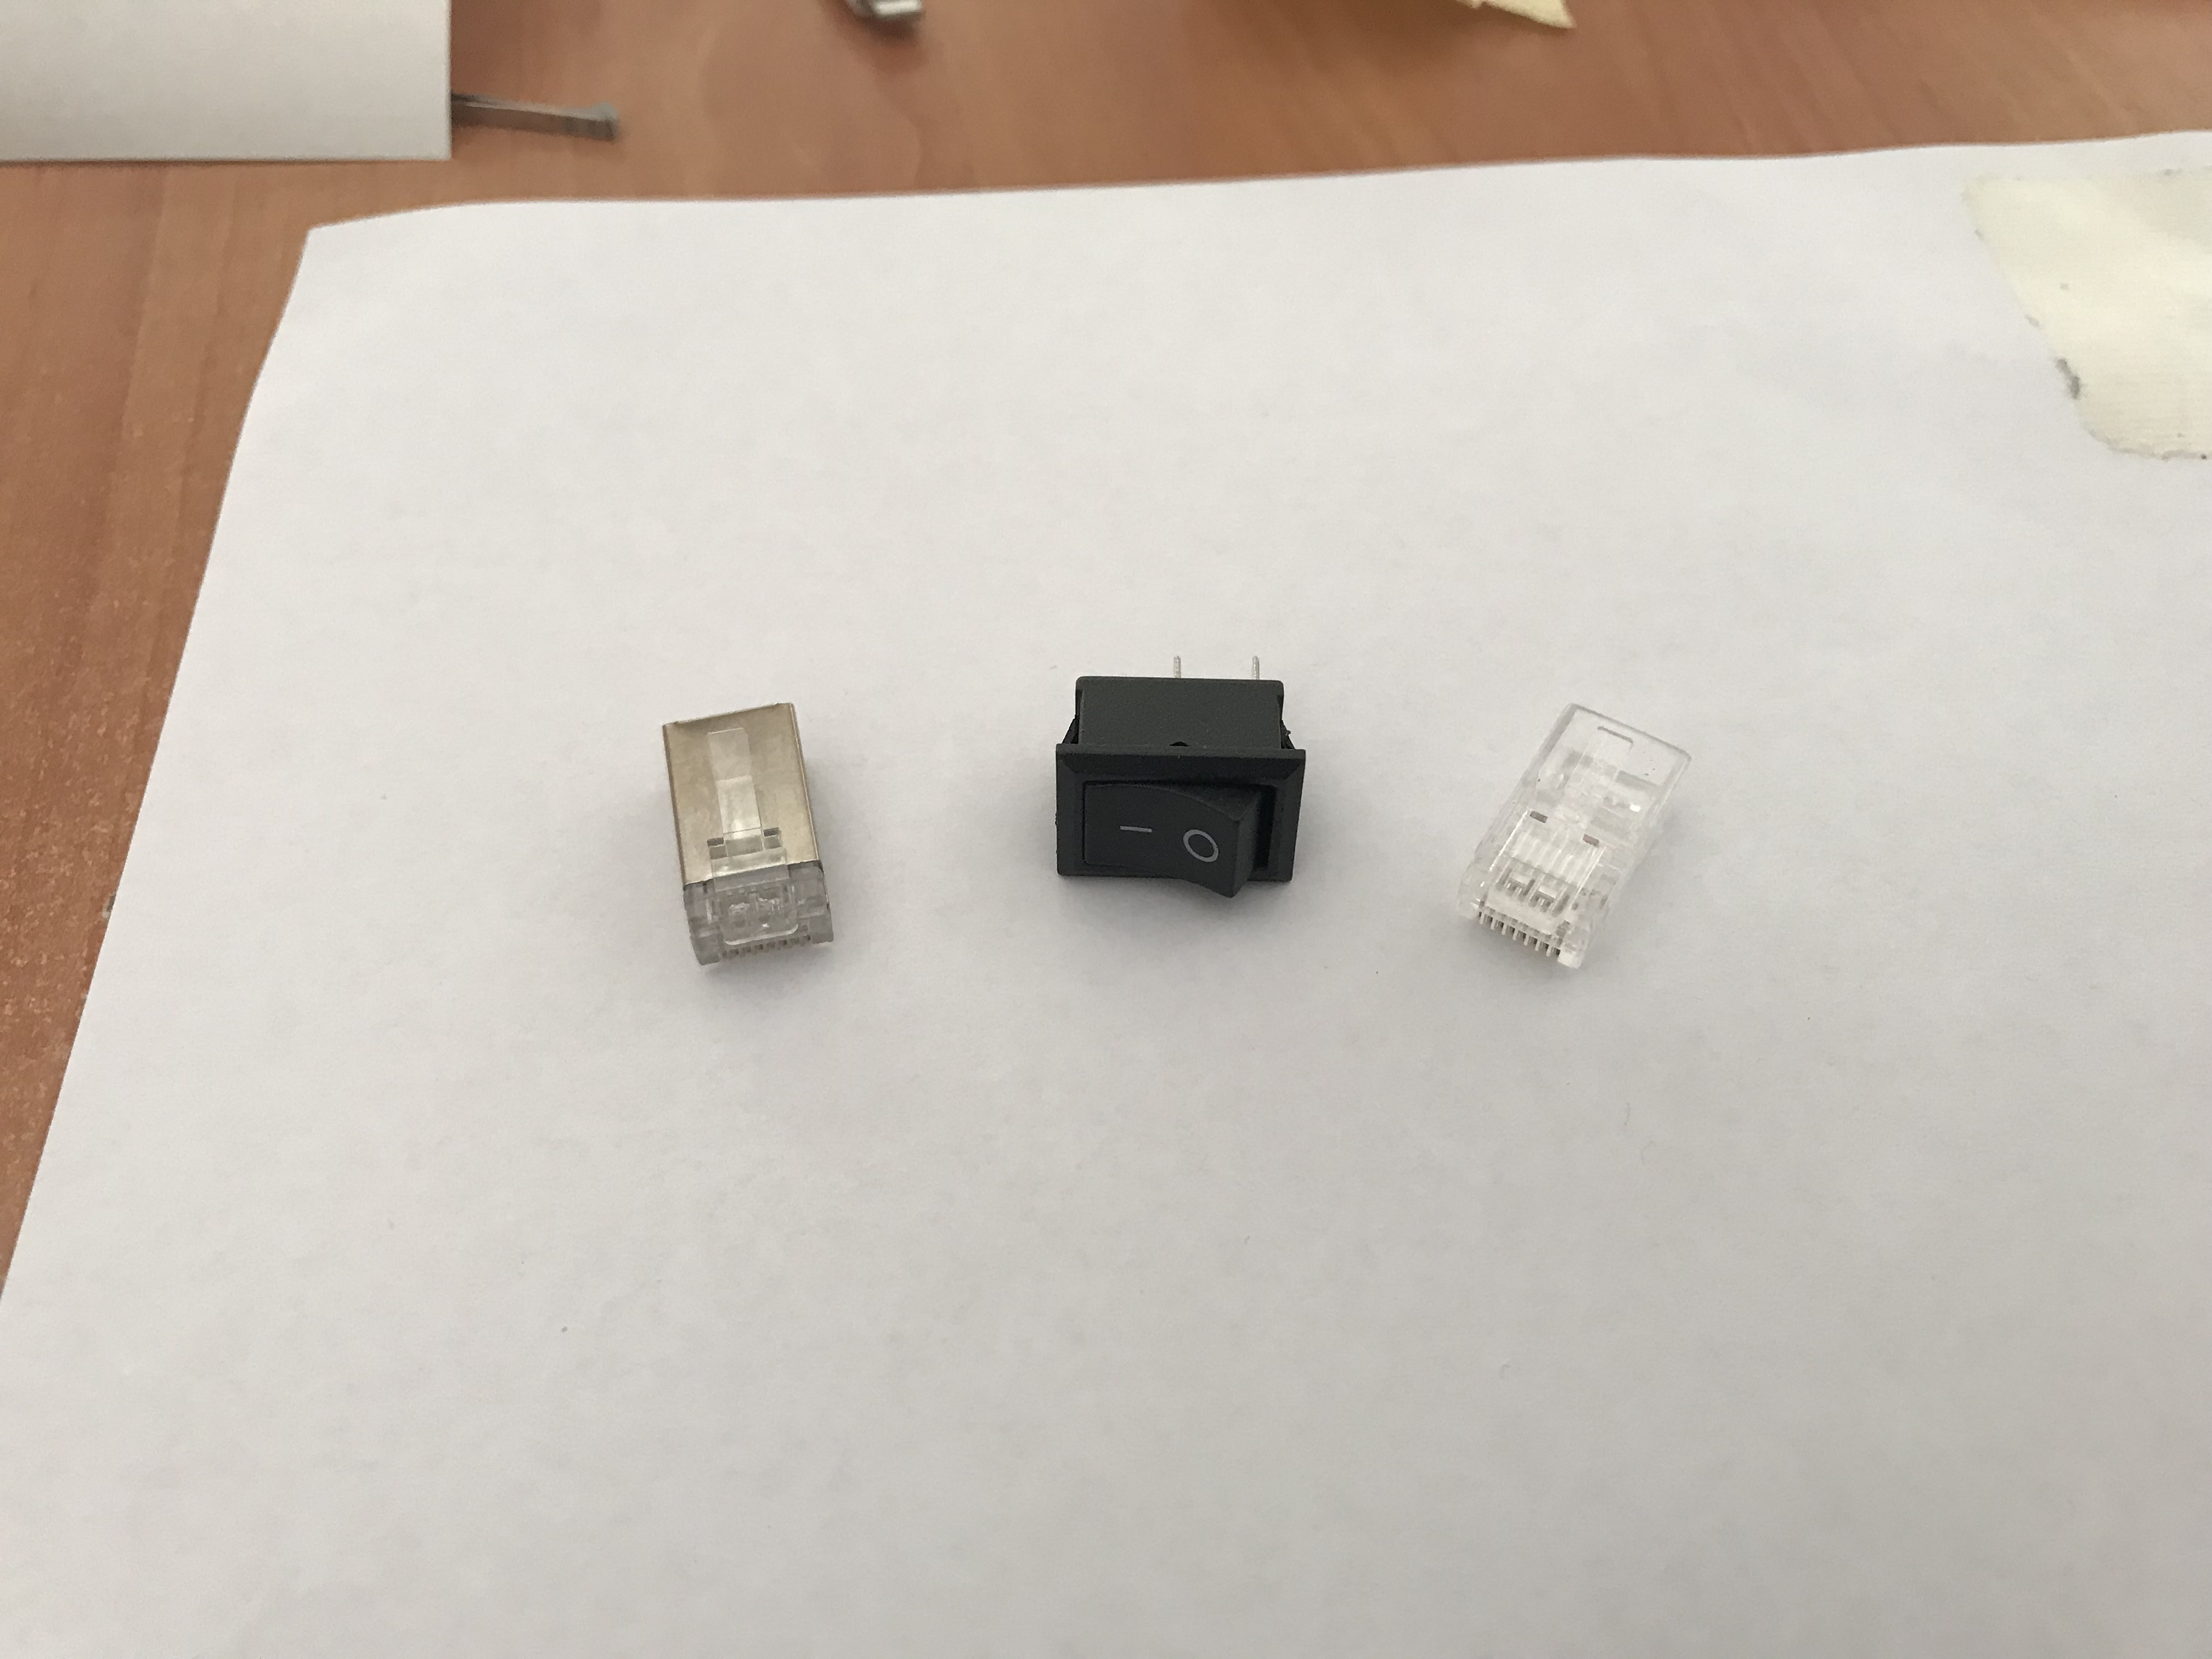
\includegraphics[scale=.1]{pictures/rj.jpg}};
            \end{scope}
        }{
            \draw (0,0) rectangle (3,1.5) ;
        }{Amazon}{Interruptor} {125V} {10A} 
        
        \connectorinfo{Codigo}{RA11131121}{
            \tabitem \textbf{Fabricante}: E-Switch
        }
        \cline{1 - 2}
        \connectorblockinfo{Uso}{UI Dcc Decoder Config}
        \connectorblockinfo{Ubicacion}{TR}
    \end{tabular}
    \caption{Interruptor Basculante}
    \label{tab:rs-KCD1-101}
\end{table}

%Modulo Rele
\begin{table}[H]
    \centering
    \renewcommand\theadfont{\bfseries}
    \setlength{\tabcolsep}{10pt}
    \renewcommand{\arraystretch}{1.5}

    \begin{tabular}{|c|c|c|c|c|}
        \beginConnectorTable{Reles}
        \multirow{3}{*}{\makecell{Modulo 1x}}
        \connectordata{
            %\draw (0,0) rectangle  +(2.5,1.8);
            \begin{scope}
                \clip (0,0) rectangle  +(3,1.5);
                \node[inner sep=0pt] at (1.5,0.75)
                    {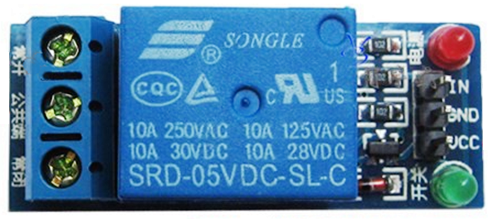
\includegraphics[scale=.3]{pictures/rele.jpg}};
            \end{scope}
        }{
            \draw (0,0) rectangle (3,1.5) ;
        }{Aliexpress}{Modulo Rele} {250V} {10A} 
        \cline{1 - 2}
        \connectorblockinfo{Uso}{Horno SMD (intencion)}
        \connectorblockinfo{Ubicacion}{TT-Tren}
    \end{tabular}
    \caption{Reles}
    \label{tab:Reles}
\end{table}